\documentclass[AMA,STIX1COL]{WileyNJD-v2}

%% my added packages
\usepackage{verbatim}
\usepackage{caption}
\usepackage{subcaption}
\usepackage{booktabs} % for nice tables
%\usepackage{breqn}
\newcommand{\ud}{\mathrm{d}}
\renewcommand{\vec}[1]{\mathbf{#1}}
\newcommand{\veca}[2]{\mathbf{#1}{#2}}
\renewcommand{\bm}[1]{\mathbf{#1}}
\newcommand{\bs}[1]{\boldsymbol{#1}}
\graphicspath{{figs/}}

\articletype{Research Article}%

\received{26 April 2016}
\revised{6 June 2016}
\accepted{6 June 2016}

\raggedbottom

\begin{document}

\title{Parallel spectral element method for guided wave based structural health monitoring\protect\thanks{Parallel spectral element method for SHM.}}

\author[1]{Pawel Kudela*}

\author[2]{Jochen Moll}

\author[1]{Piotr Fiborek }

\authormark{PAWEL KUDELA \textsc{et al}}


\address[1]{\orgdiv{Institute of Fluid Flow Machinery}, \orgname{Polish Academy of Sciences}, \orgaddress{\state{80-231 Gdansk}, \country{Poland}}}

\address[2]{\orgdiv{Department of Physics}, \orgname{J.W. Goethe--University}, \orgaddress{\state{60438 Frankfurt}, \country{Germany}}}


\corres{*Pawel Kudela,  \email{pk@imp.gda.pl}}

%\presentaddress{This is sample for present address text this is sample for present address text}

\abstract[Summary]{Parallel implementation of spectral element method is developed in which flat shell spectral elements are utilized for spatial domain representation. The implementation is realised by using Matlab Parallel Computing Toolbox and optimized for Graphics Processing Unit (GPU) computation. In this way, considerable computation speedup can be achieved in comparison to computation on conventional processors. The implementation includes interpolation of wavefield on a uniform grid. The method was tested on experimental data set available on Open Guided Waves platform. Qualitative comparison was performed on full wavefield data, whereas quantitative comparison was made directly on signals of propagating Lamb waves registered by piezoelectric transducers. In both cases, good agreement between numerical and experimental results was achieved. The proposed method is particularly useful for structural health monitoring algorithms in which signal parameters are required such as wave velocity dependence on angle of propagation. Moreover, it enables model--assisted damage size estimation in which damage influence curve is estimated based on large numerical data set and sparse experimental data. Due to relatively short computation time, large data sets can be generated and used for machine learning or other soft computing methods opening up new possibilities in health monitoring of metallic and composite structures.}

\keywords{spectral element method, guided waves, parallel implementation, delamination, GPU computation, Open Guided Waves}

\jnlcitation{\cname{%
\author{Kudela P.}, 
\author{J. Moll}, and
\author{P. Fiborek}, 
} (\cyear{2019}), 
\ctitle{Parallel spectral element method for guided wave based structural health monitoring}, \cjournal{International Journal for Numerical Methods in Engineering}, \cvol{2019;00:00--00}.}

\maketitle

\footnotetext{\textbf{Abbreviations:} SHM, structural health monitoring; GPU, Graphics Processing Unit; CUDA, Compute Unified Device Architecture}


\section{Introduction}\label{sec1}

	Guided waves are very often utilized in nondestructive evaluation and structural health monitoring. There are many algorithms based on ultrasound signals registered by piezoelectric sensors able to predict if a structure is damaged and where the damage is located. However, they often require information about wave velocity or other parameters which must be provided from a model. For example in anisotropic composite laminates the wave velocity of particular mode depends on angle of propagation. Improper velocity values would lead to wrong identification of damage location.  Moreover, it is very difficult to implement signal processing algorithm for damage size estimation exclusively based on experimental signals. Usually model--assisted approach is required supported by comprehensive numerical simulations. Unfortunately, due to complex multimodal and dispersive nature of guided waves, wave propagation modelling is very challenging. 

Guided wave modelling techniques can be roughly divided into analytic, semi--analytic and approximate in which domains are discretized in various ways e.g. finite element method. Analytic methods are suitable for parametric studies and can be used for damage influence analysis in simple isotropic structures~\cite{Giurgiutiu2014}. Semi--analytic methods such as semi-analytic finite element (SAFE) method is utilized for dispersion curves analysis and wave attenuation in wave guides of arbitrary cross-sections including multi-layer composite laminates~\cite{Bartoli2006}. Another method which utilizes analytic solution of wave equation as a shape function is the frequency domain spectral finite element method. The method was popularized by Doyle~\cite{Doyle1989} and exploited by many researchers~\cite{RoyMahapatra2003,Palacz2005} mostly in relation to wave propagation analysis in 1D waveguides. The advantage of the method is that it is very fast if only few response points are considered and guided waves of high frequency can be modelled easily. On the other hand, the periodic nature of Fourier transform and inverse Fourier transform used in this method in conjunction with finite dimensions of waveguide causes that artificial wave packets appears in signal responses. Special \emph{throw-off elements} can be applied at ends of 1D waveguides to alleviate this problem~\cite{Doyle1989}. In 2D waveguides such as membranes and plates the method has been extended to wavelet spectral finite element method~\cite{Mitra2008,Yang2016}. It should be noted that by using this approach simulation of wave propagation in anisotropic materials with defects can be conducted.

An interesting approximate method was proposed by Joulaian et al., namely spectral cell method~\cite{Joulaian2014}. The main idea of the method is to embed physical domain into a bigger domain 
that can be easily meshed into a Cartesian grid consisting of rectangular cells, i.e. quadrilaterals
in 2D or hexahedrals in 3D, respectively. It can be efficient in combination with octree meshing and explicit time integration. The authors applied the method for simulating wave propagation in complex structures made of heterogeneous materials. Recently, the code was adapted for the use on multiple GPUs and CPUs~\cite{Mossaiby2019}. 

Willberg et al.~\cite{Willberg2012} studied several higher order finite element methods with polynomial degrees \emph{p}{\textgreater}2. The results highlight the superiority of higher order approaches in comparison to low order (linear, quadratic) finite elements. The convergence behaviour is more rapid and considerably less degrees of freedom are needed for accurate results.

Another higher order method is the time domain spectral element method (SEM). It is characterized by fast convergence rate, diagonality of mass matrix and high parallelism of the code. The SEM was originally developed by Patera in 1984 for modelling of laminar flows~\cite{Patera1984}. Than, over the years the method has gained attention in geophysics community for the numerical simulation of seismic wave propagation~\cite{Seriani1998,Komatitsch2009}. The method was later adopted for modelling structural health monitoring systems based on anomalies of guided waves~\cite{Schulte2010,Ostachowicz2012,Lonkar2013}. 

Leckey et al.~\cite{Leckey2018} investigated four numerical simulation tools: custom implementation~\cite{Leckey2014} of the 3D Elastodynamic Finite Integration Technique (EFIT) \cite{Schubert1998} along with three widely used commercial finite element codes: COMSOL, ABAQUS, and ANSYS. The studied example was related to interaction of propagating Lamb waves with delamination in cross-ply laminate consisted of 8 layers (delamination was below second ply counting from the top). The laminate was modelled by dense mesh of 3D solid elements. The numerical results were compared with experiment in terms of wavefield showing quite good agreement in case of some methods. Unfortunately, despite the simulations were performed on a workstation equipped with 16 cores, the efficiency of each investigated methods is so low that it is prohibitive to perform any parametric study or generate data sets e.g. for machine learning (the shortest simulation run time was for the case of COMSOL i.e. 19.5~hours followed by ABAQUS implicit i.e. 40~hours).

High computation demanding of guided wave propagation problem causes that more and more researchers have been looking for possible ways of computation speedup over last decade. One of possible popular solution is by using parallelisation via the Compute Unified Device Architecture (CUDA), which enables parallel computing on powerful graphic cards. A parallel algorithm of the Local Interaction Simulation Approach (LISA) for Lamb wave propagation modelling in aluminum plates exposed to temperature changes was developed by~Kijanka et~al.~\cite{Kijanka2013}. Similar approach to model the nonlinear dynamic interactions between ultrasonic guided waves and fatigue cracks was utilised by Shen and Cesnik~\cite{Shen2017}.  

The presented in this paper method for solving guided wave propagation problems combines high order time domain spectral element method (SEM) with CUDA through Matlab Parallel Computing Toolbox. The presented concept of parallel implementation of SEM is similar to the parallel implementation developed previously~\cite{Kudela2016} but it is applied to flat shell spectral elements instead of 3D solid elements. Moreover, it is more suitable for wave propagation modelling in multilayer composite laminates because it leads to much lower number of degrees of freedom. Therefore, the computation can be performed faster which is important for application in the model--assisted structural health monitoring. The implementation includes interpolation of the wavefield from top or bottom surface of a flat shell on a uniform grid of points. In this way wavefield data processing and visualisation can be performed easily. The method was tested for the first time on experimental data set available on Open Guided Waves platform.

\section{Numerical modelling}
\subsection{Flat shell spectral element (theoretical background)}
The developed spectral finite element for flat shell modelling is based on Mindlin--Reissner first order shear deformation theory. It has 36 nodes and 5 degrees of freedom in each node: displacement components $u_0$ and $v_0$ in neutral plane along $x$ and $y$ axis, respectively, transverse displacement $w_0$ and two independent rotations of cross-section $\varphi_x(x,y)$ and $\varphi_y(x,y)$. The spectral shell element is schematically shown in Fig.~\ref{fig:spectral_shell_element}.
\begin{figure} [h!]
	\centering
	\includegraphics{shell.png}	
	\caption{36--node spectral shell element.}
	\label{fig:spectral_shell_element}
\end{figure}
The displacement field can be written as:
\begin{equation}
\begin{split}
& u(x,y,z)=u_0(x,y) - \varphi_x(x,y) \cdot z\\
& v(x,y,z)=v_0(x,y) - \varphi_y(x,y) \cdot z\\
& w(x,y,z)=w_0(x,y) \label{eq:delam_platedispl}
\end{split}
\end{equation}
The strain field assuming small deformations is:
\begin{equation}
\begin{split}
& \varepsilon_x(x,y,z)= \frac{\partial u_0}{\partial x} - \frac{\partial \varphi_x}{\partial x} \cdot z\\
& \varepsilon_y(x,y,z)=\frac{\partial v_0}{\partial y} - \frac{\partial \varphi_y}{\partial y} \cdot z\\
& \gamma_{xy}(x,y,z)= \frac{\partial u_0}{\partial y} +  \frac{\partial v_0}{\partial x} - \left( \frac{\partial \varphi_x}{\partial y} + \frac{\partial \varphi_y}{\partial x}\right)\cdot z\\
& \gamma_{yz}(x,y,z)= \frac{\partial w_0}{\partial y} - \varphi_y\\
& \gamma_{zx}(x,y,z)= \frac{\partial w_0}{\partial x} - \varphi_x 
\label{eq:delam_platestrains}
\end{split}
\end{equation}
Assuming approximation of displacement field within the element:
\begin{equation}
\left[\begin{array}{l} u_0^e(\xi, \eta) \\ \varphi_x^e(\xi, \eta)\\ v_0^e(\xi, \eta) \\ \varphi_y^e(\xi, \eta)\\ w_0^e(\xi, \eta)\\ \end{array}\right] = \bm{N}^e \vec{\hat{u}}^e = \sum \limits_{j=1}^{6} \sum \limits_{i=1}^{6} N^e_i(\xi) N^e_i(\eta)\, \bm{I} \left[ \begin{array}{l} {\hat{u}_0}^e(\xi_i,\eta_j)\\\hat{\varphi}_x^e(\xi_i,\eta_j)\\{\hat{v}_0}^e(\xi_i,\eta_j) \\\hat{\varphi}_y^e(\xi_i,\eta_j) \\ \hat{w}_0^e(\xi_i,\eta_j)\end{array} \right]\label{eq:delam_plateaproxim}
\end{equation}  
where $\bm{N}^e$ are shape functions, $\vec{\hat{u}}^e$ are nodal degrees of freedom in the element, $\bm{I}$ is the unit matrix of the size 5x5, and assuming approximation of geometry of the element:	\begin{equation}
\left[\begin{array}{l} x_0^e(\xi, \eta) \\ y_0^e(\xi, \eta)  \end{array}\right] = \sum \limits_{j=1}^{6} \sum \limits_{i=1}^{6} N^e_i(\xi) N^e_j(\eta)\, \left[ \begin{array}{l} x^e(\xi_i,\eta_j)\\y^e(\xi_i,\eta_j)\end{array} \right]\label{eq:delam_plategeom}
\end{equation}  
and substituting into Eq.~(\ref{eq:delam_platestrains}) one can obtain approximated strains: 
\begin{equation}
\bs{\varepsilon}^e(\xi,\eta) = 	\vec{B}^e \vec{\hat{u}}^e \label{eq:delam_plate_relat}
\end{equation} 
where $	\vec{B}^e$ is the matrix relating strains with nodal displacements calculated as:
\begin{equation}
\begin{split}
& \vec{B}^e =  \bm{L} \, \bm{N}^e\!(\xi,\eta) \\ 
& \bm{L} = \left[\begin{array}{ccccc} \frac{\partial}{\partial x} & -z\, \frac{\partial}{\partial x} & 0 & 0 & 0 \\[4pt]
0&0&\frac{\partial}{\partial y}&-z\, \frac{\partial}{\partial y}&0\\[4pt]
\frac{\partial}{\partial y} &-z\,\frac{\partial}{\partial y} & \frac{\partial}{\partial x} &-z\,  \frac{\partial}{\partial x} &0 \\[4pt]
0&0&0&-1&\frac{\partial}{\partial y} \\[4pt]
0&-1&0&0&\frac{\partial}{\partial x} \end{array} \right], \quad \left[\begin{array}{c}\frac{\partial }{\partial x}\\[4pt] \frac{\partial }{\partial y}\end{array}\right] = \vec{J}^{-1} \left[\begin{array}{c}\frac{\partial }{\partial \xi}\\[4pt] \frac{\partial }{\partial \eta}\end{array}\right]
\label{eq:delam_plate_disp_strains}
\end{split}
\end{equation} 
where $\vec{J}$ is Jacobi matrix which has a form:
\begin{equation}
\vec{J} = \Bigg[ \begin{array}{cc}\frac{\partial x}{\partial \xi}&\frac{\partial y}{\partial \xi}\\[4pt]
\frac{\partial x}{\partial \eta}&\frac{\partial y}{\partial \eta}\end{array} \Bigg].
\label{eq:Jacobi2D}
\end{equation}
Elemental mass matrix and stiffness matrix are calculated numerically by using Gaussa-Lobatto-Legendre (GLL) integration rule:
\begin{equation}
\begin{split}
\bm{m}^e &= \int \limits_{\Omega_e} \big[\bm{N}^e\!(x,y)\big]^{\!T} \bm{R}^e\!(x,y) \, \bm{N}^e\!(x,y) \; \ud \Omega_e \\
&	\approx \sum \limits_{j=1}^{6} \sum \limits_{i=1}^{6} w_i\, w_j \, \big[\bm{N}^e\!(\xi_i, \eta_j)\big]^{\!T} \bm{R}^e\!(\xi_i, \eta_j)	\,
\bm{N}^e\!(\xi_i,\eta_j) \, \det(\vec{J}^e)\label{eq:delam_plate_mass}
\end{split}
\end{equation} 
\begin{equation}
\begin{split}
\bm{k}^e &= \int \limits_{V_e} \big[\vec{B}^e\!(x,y)\big]^{\!T} \vec{D}^e \!(x,y)\, \vec{B}^e\!(x,y) \; \ud V_e \\
& \approx \sum \limits_{j=1}^{6} \sum \limits_{i=1}^{6} w_i\, w_j\! \int \limits_{-h/2}\limits^{h/2} \big[\vec{B}^e\!(\xi_i,\eta_j)\big]^{\!T}\, \bm{\overline Q}^e\!(\xi_i,\eta_j) \, \vec{B}^e\!(\xi_i,\eta_j) \, \det(\vec{J}^e)\, \ud z\\
&=\sum \limits_{j=1}^{6} \sum \limits_{i=1}^{6} w_i\, w_j \sum \limits_{k=1}^{N} \int_{h_{k-1}}^{h_k} \big[\vec{B}^e\!(\xi_i,\eta_j)\big]^{\!T} \bm{\overline Q}_k^e\!(\xi_i,\eta_j) \, \vec{B}^e\!(\xi_i,\eta_j) \, \det(\vec{J}^e)\, \ud z \label{eq:dealm_plate_stiffness}
\end{split}
\end{equation} 
The quadrature weight $w_i > 0$, which are independent form the element, are defined by:
\begin{equation}
w_i = \frac{2}{m(m-1)\big[ P_{m-1}\!(\xi_i) \big]^2}\; , \quad i \in 1,\ldots, m \label{eq:weights}
\end{equation}
where $P_{m-1}$ is Legendre polynomial of order $m-1$, $m=6$ for 6~$\times$~6 nodes flat shell spectral element.
Matrix $\bm{R}^e$ from Eq.~(\ref{eq:delam_plate_mass}) is calculated as:
\begin{equation}
\begin{split}
&\bm{R}^e = \left[\begin{array}{ccccc} I_0 & 0&0&0&0 \\ 0& I_2&0&0&0 \\0&0&I_0&0&0\\0&0&0&I_2&0\\ 0&0&0&0&I_0 \end{array}\right]\\
&I_0 =  \sum \limits_{k=1}\limits^{N} \rho_k \,(h_{k-1} - h_k),\\ 
& I_2 =  \sum \limits_{k=1}\limits^{N} \rho_k \,(h_{k-1}^3 - h_k^3)/3,
\label{eq:delam_plate_mass_dens}
\end{split}
\end{equation}
where $N$ -- the number of composite layers, $\rho_k$ -- mass density of $k$-th layer, $h_k$ -- the distance from the neutral surface to the top surface of the $k$-th layer, $h_{k-1}$ -- the distance from the neutral surface to the bottom surface of the $k$-th layer.
The matrix $\bm{\overline Q}_k^e$ from Eq.~(\ref{eq:dealm_plate_stiffness}) for $k$-th composite layer has a form:
\begin{equation}
\bm{\overline Q}_k^e = \left[\begin{array}{ccccc} \overline{Q}_{11} & \overline{Q}_{12}& \overline{Q}_{16} & 0&0\\[2pt]
\overline{Q}_{12}& \overline{Q}_{22} & \overline{Q}_{26}& 0&0\\\overline{Q}_{16}&\overline{Q}_{26}&\overline{Q}_{66}&0&0\\[2pt]
0& 0 &0&\overline{Q}_{44}& \overline{Q}_{45}\\[2pt]
0&0&0&\overline{Q}_{45}&\overline{Q}_{55}\end{array}\right] \label{eq:dealm_plate_stf}
\end{equation}
The components of matrix $\bm{\overline Q}_k^e$ are calculated for lamina rotated according to stacking sequence. The transformation matrix of stiffness tensor $\bm{Q}_k^e$ along with explicit formulas can be found in the literature~\cite{Vinson1987}.
It should be noted that in general both mass density $\rho_k$ as well as stiffness tensor components $\bm{Q}_k^e$ can have arbitrary values at GLL points but for simplicity it is assumed that they are constant within $k$-th layer. Integral over thickness of layers in Eq.~\ref{eq:dealm_plate_stiffness} is evaluated analytically which leads to the following constants:
\begin{equation}
\begin{split}
& A_{ij} =  \sum \limits_{k=1}\limits^{N} (\overline{Q}_k)_{ij} \,(h_{k-1} - h_k),\quad i,j = 1,2,6,\\
& A_{ij} =  \sum \limits_{k=1}\limits^{N} (\overline{Q}_k)_{ij} \,5/4 (h_{k-1} - h_k - 4/3 (h_{k-1}^3 - h_k^3)/h^2 ),\quad i,j = 4,5,\\
& B_{ij} = \sum \limits_{k=1}\limits^{N}(\overline{Q}_k)_{ij} \,(h_{k-1}^2 - h_k^2)/2, \quad i,j = 1,2,6,\\
& D_{ij} = \sum \limits_{k=1}\limits^{N}(\overline{Q}_k)_{ij} \,(h_{k-1}^3 - h_k^3)/3, \quad i,j = 1,2,6,
\end{split}
\end{equation}
where $h$ is the total shell thickness.
\vspace{0.5cm}
\subsection{Implementation by using vectorization of the code and Matlab Parallel Computing Toolbox}
In classic finite element approach elemental matrices are assembled to form equation of motion:
\begin{equation}
\bm{M} \vec{\ddot{U}} + \bm{C} \vec{\dot{U}} + \bm{K} \vec{U} = \vec{F} \label{eq:motion}
\end{equation}  
where $ \bm{M} $ is the global mass (inertia) matrix, $ \bm{K} $ is the global stiffness matrix,  $\bm{C} $ is the global damping matrix, $\vec{U}$ is the vector of global degrees of freedom and~$\vec{F}$ is the vector of the time dependent excitation (in this particular case the vector of equivalent piezoelectric forces). The most efficient way to solve the Eq.~\ref{eq:motion} is by using explicit integration scheme. Assuming the following approximations:
\begin{equation}
\ddot{\vec{U}}\simeq \frac{1}{\Delta t^2} \left(\vec{u}_{t+\Delta t} - 2\,\vec{u}_t + \vec{u}_{t-\Delta t}\right) \label{eq:central_scheme}
\end{equation}
\begin{equation}
\dot{\vec{U}}\simeq \frac{\vec{u}_{t+\Delta t} -\vec{u}_{t-\Delta t}}{2 \Delta t}
\label{eq:first_derivative_scheme}
\end{equation}
and substituting Eq.~\ref{eq:central_scheme}-\ref{eq:first_derivative_scheme} into Eq.~\ref{eq:motion} leads to:
\begin{equation}
\begin{split}
\underbrace{\left(\frac{1}{\Delta t^2} \,\bm{M} + \frac{1}{2 \Delta t} \bm{C}\right)}_{\vec{M}_0} \vec{u}_{t+\Delta t} &= \vec{F}_t - \underbrace{\left(\bm{K} \vec{u}_t\right)}_{\vec{F}^i} + \underbrace{\left(\frac{2}{\Delta t^2} \,\bm{M} \right)}_{\vec{M}_1}\vec{u}_t \\
&+ \underbrace{\left(- \frac{1}{\Delta t^2} \,\bm{M} + \frac{1}{2 \Delta t} \bm{C}\right)}_{\vec{M}_2} \vec{u}_{t-\Delta t}.
\label{eq:explicit_integration}
\end{split}
\end{equation}
The advantage of the spectral element method over finite element method is that the mass matrix is diagonal. It has been shown that for the Lamb wave attenuation modelling it is possible to assume that the damping matrix is proportional to mass matrix~\cite{Wandowski2017}. In such case calculation of displacements at the time step $t + \Delta t$ is straightforward and does not require costly matrix inversion. However, the term $\vec{F}^i=\bm{K}\vec{u}_t$ related to internal forces at the time step $t$ is still computationally intensive. Moreover, assembly of the stiffness matrix is troublesome because it requires a lot of memory and limits the size of wave propagation problem which can be simulated. In order to alleviate these deficiencies, parallel code is proposed in which assembly is performed at the internal force vector level without necessity of stiffness matrix assembly. The proposed approach is very similar to the parallel implementation given in~\cite{Kudela2016}. However, due to analytic integration over thickness and more complex displacement field in comparison to 3D solid spectral elements, the process of calculation of the term $\vec{F}^i=\bm{K}\vec{u}_t$ is different and it is divided into two steps. In the first step stress-like components are calculated at the time moment $t$ (index $t$ in displacement vectors is omitted for clarity):
\begin{equation}
\begin{split}
\bs{\sigma}_{xx}&=\left((\bm{N},_{\xi}\vec{U}_x).*(\vec{J}^{-1})_{11}+(\bm{N},_{\eta}\vec{U}_x).*(\vec{J}^{-1})_{21}\right).*\vec{A}_{11}\\
&+\left((\bm{N},_{\xi}\bs{\Phi}_x).*(\vec{J}^{-1})_{11}+(\bm{N},_{\eta}\bs{\Phi}_x).*(\vec{J}^{-1})_{21}\right).*\vec{B}_{11}\\
&+\left((\bm{N},_{\xi}\vec{U}_y).*(\vec{J}^{-1})_{12}+(\bm{N},_{\eta}\vec{U}_y).*(\vec{J}^{-1})_{22}\right).*\vec{A}_{12}\\
&+\left((\bm{N},_{\xi}\bs{\Phi}_y).*(\vec{J}^{-1})_{12}+(\bm{N},_{\eta}\bs{\Phi}_y).*(\vec{J}^{-1})_{22}\right).*\vec{B}_{12}\\
&+\left((\bm{N},_{\xi}\vec{U}_x).*(\vec{J}^{-1})_{12}+(\bm{N},_{\eta}\vec{U}_x).*(\vec{J}^{-1})_{22}\right).*\vec{A}_{16}\\
&+\left((\bm{N},_{\xi}\bs{\Phi}_x).*(\vec{J}^{-1})_{12}+(\bm{N},_{\eta}\bs{\Phi}_x).*(\vec{J}^{-1})_{22}\right).*\vec{B}_{16}\\
&+\left((\bm{N},_{\xi}\vec{U}_y).*(\vec{J}^{-1})_{11}+(\bm{N},_{\eta}\vec{U}_y).*(\vec{J}^{-1})_{21}\right).*\vec{A}_{16}\\
&+\left((\bm{N},_{\xi}\bs{\Phi}_y).*(\vec{J}^{-1})_{11}+(\bm{N},_{\eta}\bs{\Phi}_y).*(\vec{J}^{-1})_{21}\right).*\vec{B}_{16},
\end{split}
\end{equation}
\begin{equation}
\begin{split}
\bs{\sigma}_{xxz}&=\left((\bm{N},_{\xi}\vec{U}_x).*(\vec{J}^{-1})_{11}+(\bm{N},_{\eta}\vec{U}_x).*(\vec{J}^{-1})_{21}\right).*\vec{B}_{11}\\
&+\left((\bm{N},_{\xi}\bs{\Phi}_x).*(\vec{J}^{-1})_{11}+(\bm{N},_{\eta}\bs{\Phi}_x).*(\vec{J}^{-1})_{21}\right).*\vec{D}_{11}\\
&+\left((\bm{N},_{\xi}\vec{U}_y).*(\vec{J}^{-1})_{12}+(\bm{N},_{\eta}\vec{U}_y).*(\vec{J}^{-1})_{22}\right).*\vec{B}_{12}\\
&+\left((\bm{N},_{\xi}\bs{\Phi}_y).*(\vec{J}^{-1})_{12}+(\bm{N},_{\eta}\bs{\Phi}_y).*(\vec{J}^{-1})_{22}\right).*\vec{D}_{12}\\
&+\left((\bm{N},_{\xi}\vec{U}_x).*(\vec{J}^{-1})_{12}+(\bm{N},_{\eta}\vec{U}_x).*(\vec{J}^{-1})_{22}\right).*\vec{B}_{16}\\
&+\left((\bm{N},_{\xi}\bs{\Phi}_x).*(\vec{J}^{-1})_{12}+(\bm{N},_{\eta}\bs{\Phi}_x).*(\vec{J}^{-1})_{22}\right).*\vec{D}_{16}\\
&+\left((\bm{N},_{\xi}\vec{U}_y).*(\vec{J}^{-1})_{11}+(\bm{N},_{\eta}\vec{U}_y).*(\vec{J}^{-1})_{21}\right).*\vec{B}_{16}\\
&+\left((\bm{N},_{\xi}\bs{\Phi}_y).*(\vec{J}^{-1})_{11}+(\bm{N},_{\eta}\bs{\Phi}_y).*(\vec{J}^{-1})_{21}\right).*\vec{D}_{16},
\end{split}
\end{equation}
\begin{equation}
\begin{split}
\bs{\sigma}_{xy}&=\left((\bm{N},_{\xi}\vec{U}_x).*(\vec{J}^{-1})_{11}+(\bm{N},_{\eta}\vec{U}_x).*(\vec{J}^{-1})_{21}\right).*\vec{A}_{16}\\
&+\left((\bm{N},_{\xi}\bs{\Phi}_x).*(\vec{J}^{-1})_{11}+(\bm{N},_{\eta}\bs{\Phi}_x).*(\vec{J}^{-1})_{21}\right).*\vec{B}_{16}\\
&+\left((\bm{N},_{\xi}\vec{U}_y).*(\vec{J}^{-1})_{12}+(\bm{N},_{\eta}\vec{U}_y).*(\vec{J}^{-1})_{22}\right).*\vec{A}_{26}\\
&+\left((\bm{N},_{\xi}\bs{\Phi}_y).*(\vec{J}^{-1})_{12}+(\bm{N},_{\eta}\bs{\Phi}_y).*(\vec{J}^{-1})_{22}\right).*\vec{B}_{26}\\
&+\left((\bm{N},_{\xi}\vec{U}_x).*(\vec{J}^{-1})_{12}+(\bm{N},_{\eta}\vec{U}_x).*(\vec{J}^{-1})_{22}\right).*\vec{A}_{66}\\
&+\left((\bm{N},_{\xi}\bs{\Phi}_x).*(\vec{J}^{-1})_{12}+(\bm{N},_{\eta}\bs{\Phi}_x).*(\vec{J}^{-1})_{22}\right).*\vec{B}_{66}\\
&+\left((\bm{N},_{\xi}\vec{U}_y).*(\vec{J}^{-1})_{11}+(\bm{N},_{\eta}\vec{U}_y).*(\vec{J}^{-1})_{21}\right).*\vec{A}_{66}\\
&+\left((\bm{N},_{\xi}\bs{\Phi}_y).*(\vec{J}^{-1})_{11}+(\bm{N},_{\eta}\bs{\Phi}_y).*(\vec{J}^{-1})_{21}\right).*\vec{B}_{66},
\end{split}
\end{equation}
\begin{equation}
\begin{split}
\bs{\sigma}_{xyz}&=\left((\bm{N},_{\xi}\vec{U}_x).*(\vec{J}^{-1})_{11}+(\bm{N},_{\eta}\vec{U}_x).*(\vec{J}^{-1})_{21}\right).*\vec{B}_{16}\\
&+\left((\bm{N},_{\xi}\bs{\Phi}_x).*(\vec{J}^{-1})_{11}+(\bm{N},_{\eta}\bs{\Phi}_x).*(\vec{J}^{-1})_{21}\right).*\vec{D}_{16}\\
&+\left((\bm{N},_{\xi}\vec{U}_y).*(\vec{J}^{-1})_{12}+(\bm{N},_{\eta}\vec{U}_y).*(\vec{J}^{-1})_{22}\right).*\vec{B}_{26}\\
&+\left((\bm{N},_{\xi}\bs{\Phi}_y).*(\vec{J}^{-1})_{12}+(\bm{N},_{\eta}\bs{\Phi}_y).*(\vec{J}^{-1})_{22}\right).*\vec{D}_{26}\\
&+\left((\bm{N},_{\xi}\vec{U}_x).*(\vec{J}^{-1})_{12}+(\bm{N},_{\eta}\vec{U}_x).*(\vec{J}^{-1})_{22}\right).*\vec{B}
_{66}\\
&+\left((\bm{N},_{\xi}\bs{\Phi}_x).*(\vec{J}^{-1})_{12}+(\bm{N},_{\eta}\bs{\Phi}_x).*(\vec{J}^{-1})_{22}\right).*\vec{D}_{66}\\
&+\left((\bm{N},_{\xi}\vec{U}_y).*(\vec{J}^{-1})_{11}+(\bm{N},_{\eta}\vec{U}_y).*(\vec{J}^{-1})_{21}\right).*\vec{B}_{66}\\
&+\left((\bm{N},_{\xi}\bs{\Phi}_y).*(\vec{J}^{-1})_{11}+(\bm{N},_{\eta}\bs{\Phi}_y).*(\vec{J}^{-1})_{21}\right).*\vec{D}_{66},
\end{split}
\end{equation}
\begin{equation}
\begin{split}
\bs{\sigma}_{yy}&=\left((\bm{N},_{\xi}\vec{U}_x).*(\vec{J}^{-1})_{11}+(\bm{N},_{\eta}\vec{U}_x).*(\vec{J}^{-1})_{21}\right).*\vec{A}_{12}\\
&+\left((\bm{N},_{\xi}\bs{\Phi}_x).*(\vec{J}^{-1})_{11}+(\bm{N},_{\eta}\bs{\Phi}_x).*(\vec{J}^{-1})_{21}\right).*\vec{B}_{12}\\
&+\left((\bm{N},_{\xi}\vec{U}_y).*(\vec{J}^{-1})_{12}+(\bm{N},_{\eta}\vec{U}_y).*(\vec{J}^{-1})_{22}\right).*\vec{A}_{22}\\
&+\left((\bm{N},_{\xi}\bs{\Phi}_y).*(\vec{J}^{-1})_{12}+(\bm{N},_{\eta}\bs{\Phi}_y).*(\vec{J}^{-1})_{22}\right).*\vec{B}_{22}\\
&+\left((\bm{N},_{\xi}\vec{U}_x).*(\vec{J}^{-1})_{12}+(\bm{N},_{\eta}\vec{U}_x).*(\vec{J}^{-1})_{22}\right).*\vec{A}_{26}\\
&+\left((\bm{N},_{\xi}\bs{\Phi}_x).*(\vec{J}^{-1})_{12}+(\bm{N},_{\eta}\bs{\Phi}_x).*(\vec{J}^{-1})_{22}\right).*\vec{B}_{26}\\
&+\left((\bm{N},_{\xi}\vec{U}_y).*(\vec{J}^{-1})_{11}+(\bm{N},_{\eta}\vec{U}_y).*(\vec{J}^{-1})_{21}\right).*\vec{A}_{26}\\
&+\left((\bm{N},_{\xi}\bs{\Phi}_y).*(\vec{J}^{-1})_{11}+(\bm{N},_{\eta}\bs{\Phi}_y).*(\vec{J}^{-1})_{21}\right).*\vec{B}_{26},
\end{split}
\end{equation}
\begin{equation}
\begin{split}
\bs{\sigma}_{yyz}&=\left((\bm{N},_{\xi}\vec{U}_x).*(\vec{J}^{-1})_{11}+(\bm{N},_{\eta}\vec{U}_x).*(\vec{J}^{-1})_{21}\right).*\vec{B}_{12}\\
&+\left((\bm{N},_{\xi}\bs{\Phi}_x).*(\vec{J}^{-1})_{11}+(\bm{N},_{\eta}\bs{\Phi}_x).*(\vec{J}^{-1})_{21}\right).*\vec{D}_{12}\\
&+\left((\bm{N},_{\xi}\vec{U}_y).*(\vec{J}^{-1})_{12}+(\bm{N},_{\eta}\vec{U}_y).*(\vec{J}^{-1})_{22}\right).*\vec{B}_{22}\\
&+\left((\bm{N},_{\xi}\bs{\Phi}_y).*(\vec{J}^{-1})_{12}+(\bm{N},_{\eta}\bs{\Phi}_y).*(\vec{J}^{-1})_{22}\right).*\vec{D}_{22}\\
&+\left((\bm{N},_{\xi}\vec{U}_x).*(\vec{J}^{-1})_{12}+(\bm{N},_{\eta}\vec{U}_x).*(\vec{J}^{-1})_{22}\right).*\vec{B}_{26}\\
&+\left((\bm{N},_{\xi}\bs{\Phi}_x).*(\vec{J}^{-1})_{12}+(\bm{N},_{\eta}\bs{\Phi}_x).*(\vec{J}^{-1})_{22}\right).*\vec{D}_{26}\\
&+\left((\bm{N},_{\xi}\vec{U}_y).*(\vec{J}^{-1})_{11}+(\bm{N},_{\eta}\vec{U}_y).*(\vec{J}^{-1})_{21}\right).*\vec{B}_{26}\\
&+\left((\bm{N},_{\xi}\bs{\Phi}_y).*(\vec{J}^{-1})_{11}+(\bm{N},_{\eta}\bs{\Phi}_y).*(\vec{J}^{-1})_{21}\right).*\vec{D}_{26},
\end{split}
\end{equation}
\begin{equation}
\begin{split}
\bs{\sigma}_{yz}&=\left(\bs{\Phi}_y+(\bm{N},_{\xi}\vec{U}_z).*(\vec{J}^{-1})_{12}+(\bm{N},_{\eta}\vec{U}_z).*(\vec{J}^{-1})_{22}\right).*\vec{A}_{44}\\
&+\left(\bs{\Phi}_x+(\bm{N},_{\xi}\vec{U}_z).*(\vec{J}^{-1})_{11}+(\bm{N},_{\eta}\vec{U}_z).*(\vec{J}^{-1})_{21}\right).*\vec{A}_{45},\\
\bs{\sigma}_{xz}&=\left(\bs{\Phi}_y+(\bm{N},_{\xi}\vec{U}_z).*(\vec{J}^{-1})_{12}+(\bm{N},_{\eta}\vec{U}_z).*(\vec{J}^{-1})_{22}\right).*\vec{A}_{45}\\
&+\left(\bs{\Phi}_x+(\bm{N},_{\xi}\vec{U}_z).*(\vec{J}^{-1})_{11}+(\bm{N},_{\eta}\vec{U}_z).*(\vec{J}^{-1})_{21}\right).*\vec{A}_{55},
\end{split}
\end{equation}
where $.*$ denotes element-wise operation known as Hadamarad product (the same symbol for element-wise operation is used in Matlab). It should be noted that $\vec{A}$, $\vec{B}$, $\vec{D}$ and $(\vec{J}^{-1})$ with appropriate indexes are arranged in the form of vectors respective to GLL nodes of consecutive disjoint spectral elements. The same rules of disjoint arrangement are applied for nodal displacements:
\begin{equation}
\vec{U}_x = \left[
\begin{array}{c}  
\hat{\vec{u}}_0^{e=1}  \\[2pt]
\hat{\vec{u}}_0^{e=2} \\[2pt]
\vdots\\[2pt]
\hat{\vec{u}}_0^{e=n}\\[2pt]
\end{array}\right],
\quad
\vec{U}_y = \left[
\begin{array}{c}  
\hat{\vec{v}}_0^{e=1}  \\[2pt]
\hat{\vec{v}}_0^{e=2} \\[2pt]
\vdots\\[2pt]
\hat{\vec{v}}_0^{e=n}\\[2pt]
\end{array}\right],
\quad
\vec{U}_z = \left[
\begin{array}{c}  
\hat{\vec{w}}_0^{e=1}  \\[2pt]
\hat{\vec{w}}_0^{e=2} \\[2pt]
\vdots\\[2pt]
\hat{\vec{w}}_0^{e=n}\\[2pt]
\end{array}\right],
\end{equation}
\begin{equation}
\bs{\Phi}_x = \left[
\begin{array}{c}  
\hat{\bs{\varphi}}_x^{e=1}  \\[2pt]
\hat{\bs{\varphi}}_x^{e=2} \\[2pt]
\vdots\\[2pt]
\hat{\bs{\varphi}}_x^{e=n}\\[2pt]
\end{array}\right],
\quad
\bs{\Phi}_y = \left[
\begin{array}{c}  
\hat{\bs{\varphi}}_y^{e=1}  \\[2pt]
\hat{\bs{\varphi}}_y^{e=2} \\[2pt]
\vdots\\[2pt]
\hat{\bs{\varphi}}_y^{e=n}\\[2pt]
\end{array}\right],
\end{equation}
where $n$ is the total number of elements in the spectral element mesh. Sparse matrices of shape function derivatives are formed in similar way, i.e.:
\begin{equation}
\bm{N},_{\xi} = \left[
\begin{array}{cccc}  
\bm{N},_{\xi}^{e=1} & 0 & \ldots & 0\\[2pt]
0& \bm{N},_{\xi}^{e=2}  & \ldots& 0\\[2pt]
\vdots&\vdots&\ddots&0\\[2pt]
0& 0 &0&\bm{N},_{\xi}^{e=n}\\[2pt]
\end{array}\right].
\end{equation}
In the second step internal forces are calculated on the degree of freedom level: 
\begin{equation}
\begin{split}
\vec{F}_u^i&=\bm{N},_{\xi}^T \left(\bs{\sigma}_{xx}\,.*(\vec{J}^{-1})_{11}\,.*\vec{W}\right)+\bm{N},_{\eta}^T \left(\bs{\sigma}_{xx}\,.*(\vec{J}^{-1})_{21}\,.*\vec{W}\right)\\
&+\bm{N},_{\xi}^T \left(\bs{\sigma}_{xy}\,.*(\vec{J}^{-1})_{12}\,.*\vec{W}\right)+\bm{N},_{\eta}^T \left(\bs{\sigma}_{xy}\,.*(\vec{J}^{-1})_{22}\,.*\vec{W}\right), \\ 
\vec{F}_v^i&=\bm{N},_{\xi}^T \left(\bs{\sigma}_{yy}\,.*(\vec{J}^{-1})_{12}\,.*\vec{W}\right)+\bm{N},_{\eta}^T \left(\bs{\sigma}_{yy}\,.*(\vec{J}^{-1})_{22}\,.*\vec{W}\right)\\
&+\bm{N},_{\xi}^T \left(\bs{\sigma}_{xy}\,.*(\vec{J}^{-1})_{11}\,.*\vec{W}\right)+\bm{N},_{\eta}^T \left(\bs{\sigma}_{xy}\,.*(\vec{J}^{-1})_{21}\,.*\vec{W}\right),\\
\vec{F}_w^i&=\bm{N},_{\xi}^T \left(\bs{\sigma}_{yz}\,.*(\vec{J}^{-1})_{12}\,.*\vec{W}\right)+\bm{N},_{\eta}^T \left(\bs{\sigma}_{yz}\,.*(\vec{J}^{-1})_{22}\,.*\vec{W}\right)\\
& +\bm{N},_{\xi}^T \left(\bs{\sigma}_{xz}\,.*(\vec{J}^{-1})_{11}\,.*\vec{W}\right)+\bm{N},_{\eta}^T \left(\bs{\sigma}_{xz}\,.*(\vec{J}^{-1})_{21}\,.*\vec{W}\right),\\
\vec{M}_x^i&=\bm{N},_{\xi}^T \left(\bs{\sigma}_{xxz}\,.*(\vec{J}^{-1})_{11}\,.*\vec{W}\right)+\bm{N},_{\eta}^T \left(\bs{\sigma}_{xxz}\,.*(\vec{J}^{-1})_{21}\,.*\vec{W}\right)\\
&+\bm{N},_{\xi}^T \left(\bs{\sigma}_{xyz}\,.*(\vec{J}^{-1})_{12}\,.*\vec{W}\right)+\bm{N},_{\eta}^T \left(\bs{\sigma}_{xyz}\,.*(\vec{J}^{-1})_{22}\,.*\vec{W}\right)\\
&+\bs{\sigma}_{xz}\,.*\vec{W},\\
\vec{M}_y^i&=\bm{N},_{\xi}^T \left(\bs{\sigma}_{yyz}\,.*(\vec{J}^{-1})_{12}\,.*\vec{W}\right)+\bm{N},_{\eta}^T \left(\bs{\sigma}_{yyz}\,.*(\vec{J}^{-1})_{22}\,.*\vec{W}\right)\\
&+\bm{N},_{\xi}^T \left(\bs{\sigma}_{xyz}\,.*(\vec{J}^{-1})_{11}\,.*\vec{W}\right)+\bm{N},_{\eta}^T \left(\bs{\sigma}_{xyz}\,.*(\vec{J}^{-1})_{21}\,.*\vec{W}\right)\\
&+\bs{\sigma}_{yz}\,.*\vec{W},
\label{eq:internal_forces}
\end{split}
\end{equation}
where $^T$ is the matrix transpose and $\vec{W}$ is the vector resulting from multiplication of integration weights and Jacobian determinant at appropriate GLL points:
\begin{equation}
\vec{W} = \vec{w}_{\xi}\,.*\vec{w}_{\eta}\,.*\left(\det\vec{J}\right).
\end{equation}
Since internal forces are calculated for disjoined spectral elements, assembly of global vector $\vec{F}^i$ is necessary. It can be performed according to mesh colouring algorithm proposed in~\cite{Kudela2016}. The algorithm uniformly divides nodes of spectral elements within the whole mesh into 12 sets. Because each flat shell spectral element consists of 36 nodes, the 12 sets are of the same size so the computation can be perfectly balanced between workers or resources can be uniformly divided within one GPU card.

Once internal forces $\vec{F}^i$ are calculated and substituted into Eq.~\ref{eq:explicit_integration}, the displacements at time step $t+\Delta t$ can be explicitly obtained from perfectly vectorized code:
\begin{equation}
\vec{u}_{t+\Delta t}=1./\vec{M}_0\, .*\left(\vec{F}_t - \vec{F}^i +\vec{M}_1 \, .* \vec{u}_t +\vec{M}_2 \, .* \vec{u}_{t-\Delta t}\right),
\label{eq:vectorized_motion}
\end{equation} 
in which terms $\vec{M}_0$, $\vec{M}_1$ and $\vec{M}_2$ are stored as vectors and $./$ is element--wise division. In particular all components in Eq.~\ref{eq:internal_forces} as well as in Eq.~\ref{eq:vectorized_motion} are implemented in Matlab Parallel Computing Toolbox as \verb|gpuArray|. In this way, implementation is simple whereas CUDA GPU computation is transparent to the user. 

\subsection{Signal sensing}
Piezoelectric sensors are considered in the model in terms of stiffness and mass reduced to neutral plane of the shell. The signal sensing is realised by the following equation:
\begin{equation}
\begin{split}
\vec{s}^{pzt} &= \left[ e_{31}\left((\bm{N},_{\xi}^{pzt}\vec{U}_x^{pzt}).*(\vec{J}^{-1})_{11}^{pzt} + (\bm{N},_{\eta}^{pzt}\vec{U}_x^{pzt}).*(\vec{J}^{-1})_{12}^{pzt} \right.\right.\\
&+ \frac{h}{2} (\bm{N},_{\xi}^{pzt}\bs{\Phi}_x^{pzt}).*(\vec{J}^{-1})_{11}^{pzt} + \frac{h}{2} \left.(\bm{N},_{\eta}^{pzt}\bs{\Phi}_x^{pzt}).*(\vec{J}^{-1})_{12}^{pzt}\right)\\
&+ e_{32}\left((\bm{N},_{\xi}^{pzt}\vec{U}_y^{pzt}).*(\vec{J}^{-1})_{21}^{pzt} + (\bm{N},_{\eta}^{pzt}\vec{U}_y^{pzt}).*(\vec{J}^{-1})_{22}^{pzt} \right.\\
&+ \frac{h}{2} (\bm{N},_{\xi}^{pzt}\bs{\Phi}_y^{pzt}).*(\vec{J}^{-1})_{21}^{pzt} + \frac{h}{2} \left.\left.(\bm{N},_{\eta}^{pzt}\bs{\Phi}_y^{pzt}).*(\vec{J}^{-1})_{22}^{pzt}\right)\right] \frac{h_{pzt}}{g_{33}}, 
\end{split}
\label{eq:pzt_sensing}
\end{equation}
where $e_{31}$ and $e_{32}$ are piezoelectric coupling constants, $g_{33}$ is the extensional voltage constant, $h_{pzt}$ is the thickness of piezoelectric sensor. The submatrices and subvectors in Eq.~\ref{eq:pzt_sensing} denoted by $pzt$ superscript corresponds to nodes of appropriate spectral elements which form piezoelectric sensors. The mean value of $\vec{s}^{pzt}$ at particular integration time step gives voltage value. 
\subsection{Delamination modelling \label{sec:delam_model}}
The concept of delamination modelling is the same as in~\cite{Kudela2009}. The flat shell is divided into three regions: (I) undelaminated, (II) above delamination interface, and (III) below delamination interface. These regions are denoted in the cross--section through delamination shown in Fig.~\ref{fig:delam_modelling_shell}. 
\begin{figure} [h!]
	\centering
	\includegraphics{delam_modelling_shell.png}	
	\caption{The concept of delamination modelling: cross-section through the composite laminate and delamination showing three regions: (I) undelaminated, (II) above delamination interface, and (III) below delamination interface and corresponding elements.}
	\label{fig:delam_modelling_shell}
\end{figure}
In the flat shell all spectral elements are located at the neutral plane. There are two layers of elements at the delamination region with zero gap between them. The contact effect is neglected (penetration of nodes is allowed). It should be noted that the delamination can be placed at arbitrary interface between composite layers. The contribution to stiffness and inertia matrices is calculated separately for regions I, II and III, respectively taking into account through thickness integrals over appropriate composite layers.
	\subsection{Interpolation on a uniform grid}
With the advent of laser vibrometry technique, many algorithms for damage visualization  are developed in which full wavefield data is used. Such algorithms can be tested also on synthetic data for straightforward comparison of their efficiency. However, the mesh of spectral elements is usually unstructured due to analysed features such as delamination as well as piezoelectric transducers. Moreover, the nodes of spectral elements are non-uniformly distributed and correspond to GLL points. It makes difficult to apply damage visualization algorithms for such numerically simulated wavefields, especially when Fourier transforms are required and in turn grid of spatial points must be uniform. For this reason, interpolation technique of spectral element wavefield on uniform grid of points on top or bottom surface of the shell has been developed. 

The implemented interpolation method utilizes shape functions of spectral elements. The interpolation on uniform grid of data points is accomplished in three steps: the determination of the element containing the data point (owner element), the transformation of the data point’s coordinates into the reference coordinate system (inverse mapping), and finally the application of the spectral elements shape functions to determine the degrees of freedom at that point (Eq.~\ref{eq:delam_plateaproxim}).

In the first step, the algorithm sequentially scans the full list of spectral elements using the bounding box test. If the element fails the bounding box test, the algorithm moves to the next element in the list. If the data point is within the bounding box, the cross-product test is performed. The idea is to eliminate impossible owner elements with the computationally inexpensive bounding-box test before using the more expensive cross-product test~\cite{Silva2009}. It has been found that such implementation in case of 36--node spectral element meshes is generally faster than Matlab's \verb|inpolygon| function. 

The second step of the algorithm is inspired by the work by Li et al.~\cite{Li2014} in which inverse mapping is done iteratively. But it is modified to take into account spectral elements instead of the isoparametric hexahedral elements. As an initial point, spectral node closest to the data point in the owner element $(x_p, y_p)$ is selected. Hence, its global coordinates $(x_0, y_0)$ as well as local coordinates $(\xi_0,\eta_0)$  can be easily determined. In the first iteration inverse values of Jacobian matrix (Eq.~\ref{eq:Jacobi2D}) already stored in memory are utilized. The computation is performed for all data points in regular mesh in parallel, hence: 
\begin{equation}
\begin{split}
\bs{\xi}_{k+1}&=\bs{\xi}_k + \left(\vec{J}^{-1}_{k}\right)_{11}\,.*\left(\vec{x}_p-\vec{x}_k\right) +  \left(\vec{J}^{-1}_{k}\right)_{12}\,.*\left(\vec{y}_p-\vec{y}_k\right), \\
\bs{\eta}_{k+1}&=\bs{\eta}_k + \left(\vec{J}^{-1}_{k}\right)_{21}\,.*\left(\vec{x}_p-\vec{x}_k\right) +  \left(\vec{J}^{-1}_{k}\right)_{22}\,.*\left(\vec{y}_p-\vec{y}_k\right),
\end{split}
\label{eq:interp_initial}
\end{equation} 
in which $k=0$ in the first iteration.
Next, shape functions and Jacobians are evaluated at $(\bs{\xi}_{1}, \bs{\eta}_{1})$ points. The global coordinates of interpolated point $(x_1,y_1)$ in the owner element in the first iteration are calculated by using Eq.~\ref{eq:delam_plategeom}. Three iterations are used in the current implementation. Finally, spectral element shape functions are evaluated at interpolated local coordinates $N(\tilde{\xi}_p,\tilde{\eta}_p)$ and the wavefield is approximated by using Eq.~\ref{eq:delam_plateaproxim}.

The developed interpolation method in case of dense meshes used for wave propagation simulations is faster than Matlab embedded function \verb|griddata| which generate interpolation meshes via Delaunay triangulation. The advantage of the proposed approach is that once shape functions are evaluated at interpolated local coordinates, they are stored and used for each frame of propagating waves for wavefield interpolation whereas  \verb|griddata| function must be called for each frame separately which is inefficient.

\subsection{Computation speedup analysis}
The computational performance of the code was tested on a composite plate of material parameters introduced in section~\ref{sec:ogw}. The plate had one embedded delamination. The applied excitation was a tone-burst signal of carrier frequency 50~kHz. It was applied to the piezoelectric transducer located at the centre of the plate on the top surface. The size of the plate has been increased gradually, so that meshes contained more and more nodes (30$\times$30 cm, 40$\times$40 cm, 50$\times$50 cm, 70$\times$70 cm, 90$\times$90 cm, 100$\times$100 cm). The total run times for investigated meshes and corresponding number of degrees of freedom (NDOF) are given in Table~\ref{tab:run_time}. Computation speedup for various meshes was calculated as follows:
\begin{equation}
speedup = \frac{CPU_{time}}{GPU_{time}}
\label{eq:speedup}
\end{equation}
where $CPU_{time}$ is the average time of computation of one integration time step on a single core central
processing unit (computations were performed on a workstation equipped with 6 quad core Intel
Xeon X5660 2.8~GHz) and $GPU_{time}$ is the average time of computation of one integration time step on
GPU (computations were performed on Nvidia Tesla K20X). It can be seen in Fig.~\ref{fig:speedup} that parallel version of the code run on Tesla K20X GPU card about 5--12$\times$ faster than on single CPU (depending on the size of the problem). The trend of computation speedup is non-linear, of type $\sqrt{NDOF}$. 

\begin{table}
	\renewcommand{\arraystretch}{1.3}
	\centering \footnotesize
	\caption{Computation run times depending on the number of degrees of freedom (NDOF) for the wave propagation duration 400~$\mu$s; GPU: Nvidia Tesla K20X; CPU: Intel Xeon X5660 2.8~GHz.}
	\begin{tabular}{ccccccc} 
		%\hline
		\toprule	
		plate size [cm] & 30$\times$30  & 40$\times$40 & 50$\times$50 & 70$\times$70 & 90$\times$90 & 100$\times$100 \\
		NDOF $\cdot 10^6$ & 1.02  & 1.46 & 1.98 & 3.09 & 5.23 & 6.36 \\
		\midrule
		CPU time [h]& 4.03& 5.71 & 8.42 & 13.13 & 22.37 & 27.33\\
		\midrule
		GPU time [h]& 1.00& 1.19 & 1.26 & 1.50 & 2.00 & 2.28\\
		%\hline 
		\bottomrule 
	\end{tabular} 
	\label{tab:run_time}
\end{table}

\begin{figure} [h!]
	\centering
	\includegraphics{speedup.png}	
	\caption{Computation speedup according to Eq.~\ref{eq:speedup}; NDOF - number of degrees of freedom.}
	\label{fig:speedup}
\end{figure}
\newpage
\subsection{Potential applications}
Potential applications of the proposed model include:
\begin{itemize}
	\item model--based structural health monitoring,
	\item model--assisted structural health monitoring,
	\item benchmarking of algorithms which use guided wave signals,
	\item benchmarking of algorithms which use full wavefield data,
	\item a damage classification using machine learning.
\end{itemize}
The following differences should be noted  between the model--based and model--assisted structural health monitoring.
In the model--based approach, numerical signals must match very well experimental signals. It is because numerical signals are used in an inverse method in which certain objective function include terms such as:
\begin{equation}
g(t) = \sum_{i=1}^{N} \left(s(t)_i^{exp} - s(t)_i^{num}\right)^2,
\label{eq:obj_fun}
\end{equation}
where $s(t)^{exp}$ and $s(t)^{num}$ are experimental and numerical signals (or damage indexes), respectively.

In the model--assisted approach, on the other hand, the modelled phenomenon must reflect the real behaviour, e.g. the amplitude of transmitted wave packet decreases when the size of the damage increases. But in this case, the perfect match between numerical and experimental signals is not necessary. The aim of the presented method is model--assisted structural health monitoring.

Since it is very easy to incorporate damage into the model e.g. in the form of delamination at various locations, it makes the proposed model well suitable for benchmark data set generation. Such data set can be used for evaluation and quantitative comparison of guided wave based algorithms for damage detection and localisation in thin-walled structures (by using signals registered by sensors or full wavefield data acquired at the top or bottom surface).

Also due to reasonable computation time, it is possible to simulate thousands of examples which can be used for machine learning or in particular deep neural network training. Such soft computing methods can be used for a damage localisation, classification and size estimation. But still it will take quite a long time, e.g. 1000 simulations run for 3 hours each gives 125 days of computations on old single Nvidia Tesla K20X GPU. However, the run time can be significantly reduced by using multiple modern GPUs.

\section{Experimental validation}
\subsection{Open Guided Waves \label{sec:ogw}}
Numerical simulation were validated by using benchmark experimental data sets: Open Guided Waves (\url{http://www.open-guided-waves.de}). Open Guided Waves is an extendable online platform where high--quality and well documented datasets for guided wave--based inspections are provided~\cite{Moll2018}. The benchmark structures used for validation were quasi--isotropic carbon--fibre--reinforced polymer (CFRP) plates with embedded piezoelectric transducers. The layup was [45/0/-45/90/-45/0/45/90]\textsubscript{S}. CFRP plates had the dimensions of 500 mm $\times$ 500 mm and a thickness of 2 mm. The diameter of piezoelectric transducers was 10 mm and the thickness 0.2 mm. The specimens were based on prepreg material Hexply\textsuperscript{\textregistered} M21/34\%/UD134/T700/300. The established material properties for unidirectional Hexply material are given in Table~\ref{tab:mat_prop}. It should be added that 0$^{\circ}$ fibre orientation is along vertical edge of specimens.

Two data sets were utilized for qualitative and quantitative validation of the numerical model: "wavefield plate" and "SHM plate", respectively. The former data set consisted of full wavefield measurements of propagating guided waves excited by piezoelectric transducer placed in the centre of the plate and acquired by scanning laser Doppler vibrometer. In this case only one quarter of the plate was measured. The latter data set consisted of signals excited and registered by 12 piezoelectric sensors bonded to the surface of the plate, 6 in one row on the top and 6 in one row on the bottom (see \cite{Moll2018} for more details or compare to Fig.~\ref{fig:quad_mesh} representing the mesh used for numerical modelling). The excitation signal was a 5-cycle Hann-filtered sine wave amplified to $\pm$150~V in case of wavefield plate and  $\pm$100~V in case of SHM plate. The excitation carrier frequency was 50~kHz for wavefield measurement and 40~kHz for signals' measurement in SHM plate.
\begin{table}
	\renewcommand{\arraystretch}{1.3}
	\centering \footnotesize
	\caption{Material properties of unidirectional Hexply M21/34\%/UD134/T700/300 according to~\cite{Moll2018}; Units: GPa.}
	%\begin{tabular}{@{}ccccccc@{}} % remove spaces from vertical lines
	\begin{tabular}{cccccc} 
		%\hline
		\toprule
		$Q_{11}$ & $Q_{12}$  & $Q_{22}$ & $Q_{44}$ & $Q_{55}$ & $Q_{66}$\\
		% \cmidrule(lr){1-3} \cmidrule(lr){4-6} \cmidrule(lr){7-7}
		%\hline
		\midrule
		130& 6.1& 11.2 & 3.0 & 4.2 & 4.2\\
		%\hline 
		\bottomrule 
	\end{tabular} 
	\label{tab:mat_prop}
\end{table}
	\subsection{Defects}
In both experiments defects were simulated by an aluminium disk with a diameter of 10 mm coupled to the structure by tacky tape. The underlying idea of using this reversible damage is to provide measurement data at various places on the structure so that model-assisted probability of detection (MAPOD) techniques can be developed~\cite{Eckstein2012}. The coordinates of defects in respect to the lower left corner of the plate which has been selected for numerical model validation are given in table~\ref{tab:defect_coordinates}.

In the numerical model, two defect modelling techniques were investigated: delamination as described in section~\ref{sec:delam_model} and added mass. The delamination was modelled between 4\textsuperscript{th} and 5\textsuperscript{th} layer of composite laminate counting from the top surface.
\begin{table}
	\renewcommand{\arraystretch}{1.3}
	\centering \footnotesize
	\caption{Coordinates of analysed defects; Units: [m].}
	%\begin{tabular}{@{}ccccccc@{}} % remove spaces from vertical lines
	\begin{tabular}{cccc} 
		%\hline
		\toprule
		\multicolumn{2}{c}{\textbf{Data set I} }	& \multicolumn{2}{c}{\textbf{Data set II} } \\
		\multicolumn{2}{c}{\textbf{(wavefield plate)} }	& \multicolumn{2}{c}{\textbf{(SHM plate)} } \\
		%\midrule
		\cmidrule(lr){1-2} \cmidrule(lr){3-4}
		x & y &  x &  y  \\
		% \cmidrule(lr){1-3} \cmidrule(lr){4-6} \cmidrule(lr){7-7}
		%\hline
		0.191 & 0.145 & 0.250  & 0.427 \\ 
		%\hline 
		\bottomrule 
	\end{tabular} 
	\label{tab:defect_coordinates}
\end{table}		
\subsection{Meshing}
External meshing software GMSH~\cite{Geuzaine2009} is used for generating a mesh consisted of quadrilateral elements (see Fig.~\ref{fig:quad_mesh}). The mesh is saved in Matlab format and postprocessed by in-house code to generate spectral elements with node distribution according to GLL points. The close up of spectral element mesh near the defect is shown in Fig.~\ref{fig:spec_mesh_zoom}. 
\begin{figure} [h!]
	\centering
	%\includegraphics[width=\textwidth]{path_4_8.png}
	\includegraphics{delam_Jochen_signals_D5_a_5mm_b_5mm_angle_0added_mass.png}	
	\caption{Mesh of quadrilateral elements used in numerical modelling; red -- piezoelectric transducers; green -- defect location.}
	\label{fig:quad_mesh}
\end{figure}
\begin{figure} [h!]
	\centering
	%\includegraphics[width=\textwidth]{path_4_8.png}
	\includegraphics{delam_Jochen_signals_D5_a_5mm_b_5mm_angle_0added_mass_spec_zoom.png}	
	\caption{Close up of spectral element mesh in the damage area (green) and piezoelectric transducers no. 3 and 4.}
	\label{fig:spec_mesh_zoom}
\end{figure}
\clearpage

\subsection{Wavefield plate data set }
Comparison of experimental and numerical full wavefield data for selected time instances is presented in Fig.~\ref{fig:wavefields_comparison}. The wavefield patterns in the form of transverse velocities (see Eq.~\ref{eq:first_derivative_scheme}) are shown only for a quarter of the plate on the surface opposite to the piezoelectric actuator (bottom surface). It can be noticed that for both modelling techniques, i.e. delamination (Fig.~\ref{fig:num_frame72}, Fig.~\ref{fig:num_frame108}) and added mass (Fig.~\ref{fig:num_frame72_added_mass}, Fig.~\ref{fig:num_frame108_added_mass})	the wavefield patterns matches the experimental data very well. However, as expected, the interaction of wave front with added mass is slightly different than with delamination: the added mass interaction with the wavefront is more pronounced than in case of delamination, which is especially visible at time frame $t=112.5\,  \mu$s. The wave reflection pattern is the same in each case. It can be attributed to the fact that the added mass locally changes overall inertia and stiffness of the shell whereas delamination influences only stiffness. 

The differences between interaction of guided waves with delamination in comparison to added mass are especially visible on numerical full wavefield data collected at the top surface of the plate (see Fig.~\ref{fig:wave_entrapment}). The phenomenon of wave entrapment at defect location is present only in case of delamination (Fig.~\ref{fig:num_frame128_top}) whereas it is not present in case of added mass (Fig.~\ref{fig:num_frame128_added_mass_top}). The results related to the wave entrapment at delamination are consistent with the experimental findings available in the literature~\cite{Glushkov2012}. 

Despite these differences it seems that reversible damage in the form of added mass coupled to the structure by tacky tape is a good way for collecting benchmark data set. Such benchmark data set is a good starting point for development of algorithms based on full wavefield data for visualization of defect location even in the form of delamination.

\begin{figure} [h!]
	\begin{subfigure}[b]{0.49\textwidth}
		\centering
		% size fitted
		%\includegraphics[width=\textwidth]{SASE/\modelname_out/\modelname_angle_30_param_dispersion_curves.png}
		% size 100%
		\includegraphics[]{exp_frame64.png}
		\caption{Experiment: $t=112.5\,  \mu$s}
		\label{fig:exp_frame64}
	\end{subfigure}
	\begin{subfigure}[b]{0.49\textwidth}
		\centering
		\includegraphics[]{exp_frame100.png}
		\caption{Experiment: $t=168.7\, \mu$s}
		\label{fig:exp_frame100.png}
	\end{subfigure}
	\hfill
	\begin{subfigure}[b]{0.49\textwidth}
		\centering
		% shift of 8 frames due to excitation misalignment in experiment of pzt with (0,0) coordinates
		\includegraphics[]{Vz_1_frame72_bottom.png} 
		\caption{Simulation (delamination): $t=112.5\,  \mu$s}
		\label{fig:num_frame72}
	\end{subfigure}
	\hfill
	\begin{subfigure}[b]{0.49\textwidth}
		\centering
		\includegraphics[]{Vz_1_frame108_bottom.png}
		\caption{Simulation (delamination): $t=168.7\, \mu$s}
		\label{fig:num_frame108}
	\end{subfigure}
	\hfill
	\begin{subfigure}[b]{0.49\textwidth}
		\centering
		% shift of 8 frames due to excitation misalignment in experiment of pzt with (0,0) coordinates
		\includegraphics[]{added_mass_Vz_1_frame72_bottom.png} 
		\caption{Simulation (added mass): $t=112.5\,  \mu$s}
		\label{fig:num_frame72_added_mass}
	\end{subfigure}
	\hfill
	\begin{subfigure}[b]{0.49\textwidth}
		\centering
		\includegraphics[]{added_mass_Vz_1_frame108_bottom.png}
		\caption{Simulation (added mass): $t=168.7\, \mu$s}
		\label{fig:num_frame108_added_mass}
	\end{subfigure}
	\caption{Comparison of experimental and numerical full wavefield data.} 
	\label{fig:wavefields_comparison}
\end{figure}

\begin{figure} [h!]
	\begin{subfigure}[b]{0.49\textwidth}
		\centering
		\includegraphics[]{cut_Vz_1_frame128_top.png} 
		\caption{Simulation (delamination): $t=200\,  \mu$s}
		\label{fig:num_frame128_top}
	\end{subfigure}
	\hfill
	\begin{subfigure}[b]{0.49\textwidth}
		\centering
		\includegraphics[]{added_mass_cut_Vz_1_frame128_top.png}
		\caption{Simulation (added mass): $t=200\, \mu$s}
		\label{fig:num_frame128_added_mass_top}
	\end{subfigure}
	\caption{Comparison of numerical full wavefield data at the top surface of the plate for two defect modelling techniques: delamination and added mass. Energy trapping visible only in the case of the delamination.} 
	\label{fig:wave_entrapment}
\end{figure}
\clearpage
\subsection{SHM plate data set}
The comparison of experimental and numerical signals for selected transducer pairs is presented in Figs.~\ref{fig:path1_7}--\ref{fig:path4_8}. The transducer pair 1--7 means that the guided waves were excited in actuator 1 and registered in sensor 7 (vide Fig.~\ref{fig:quad_mesh}). The first wave packet in experimental signals should be ignored because it represents the effect of electromagnetic crosstalk.

In opposite to very good qualitative wavefield results, differences between experimental and numerical signals are evident. However, these differences are related to amplitude rather than wave velocity. It could be because of slight variation in layer thicknesses and different material damping in comparison to model. It should be also added, that both symmetric and antisymmetric wave modes are present in the signal in opposite to the wavefield measurements in which transverse wave components dominates. These wave modes overlap causing constructing or destructive interference. Wave packet positions calculated numerically matches well wave packet positions in measured signals. The slight exception is in Fig.~\ref{fig:path1_7} in which in experimental signals only one wave packet exist at about 450~$\mu$s which is actually superposition of two wave packets as numerical simulation suggest. Also at the same figure the wave packet at about 650~$\mu$s is wider in experiment than in numerical results. 

The greatest difference between experimental and numerical wave packet amplitude is in Fig.~\ref{fig:path4_8} at about 570~$\mu$s. It can be attributed to the damping coefficient selected in numerical simulation. It should be underlined that the material damping is very important because it affects attenuation of guided wave modes and in turn particular wave packets in signals. It has been assumed in the model that the damping matrix is proportional to mass matrix $\bm{C} = \alpha \bm{M}$. In the current modelling approach, the coefficient $\alpha$ was arbitrary selected ($\alpha = 4000$). However, in future some optimization technique can be applied for finding the damping coefficient so that the numerical signal best fit to experimental one. The same can be applied for optimization of elastic constants of material properties as well as piezoelectric constants. 

Another important fact is that the delamination affect signals more than added mass. This effect is especially visible in Fig.~\ref{fig:path1_7} and Fig.~\ref{fig:path2_4}. Since reversible damage in the form of added mass coupled to the structure by tacky tape affect less signals of guided waves than delamination, such signals are more challenging for signal processing methods. Therefore, it can be concluded that the experimental data set provides good benchmark for development of damage detection and localization algorithms.The next step could be comparison of variety of damage detection and localization algorithms by using the same data set.

\begin{figure} [h!]
	\centering
	%\includegraphics[width=\textwidth]{path_1_7.png}
	\includegraphics{path_1_7.png}	
	\caption{Comparison of experimental and numerical signals for transducer pairs 1--7, frequency 40~kHz.}
	\label{fig:path1_7}
\end{figure}
\begin{figure} [h!]
	\centering
	%\includegraphics[width=\textwidth]{path_2_4.png}
	\includegraphics{path_2_4.png}	
	\caption{Comparison of experimental and numerical signals for transducer pairs 2--4, frequency 40~kHz.}
	\label{fig:path2_4}
\end{figure}
\begin{figure} [h!]
	\centering
	%\includegraphics[width=\textwidth]{path_4_8.png}
	\includegraphics{path_4_8.png}	
	\caption{Comparison of experimental and numerical signals for transducer pairs 4--8, frequency 40~kHz.}
	\label{fig:path4_8}
\end{figure}
\clearpage
The conducted signal analysis leads to the conclusion that model based approach in which numerical signals are directly compared to experimental one is not feasible with the current model. However, the developed model is perfectly suited for model--assisted approaches. It is because the overall wave behaviour such as wave amplitude change due to damage and interaction of elastic waves with damage is properly modelled. It especially visible in case of differential signals presented in~Fig.~\ref{fig:path2_4_diff}. The differential signals are calculated as 'baseline' minus 'added mass' signals. The operation is performed separately for experimental and numerical signals. It can be seen that both in experimental and numerical differential signals, wave packets at about 200~$\mu$s and 400~$\mu$s gives greatest difference due to added mass. Even the amplitude of differential signals are on the same level.

\begin{figure} [h!]
	\centering
	%\includegraphics[width=\textwidth]{path_2_4_diff.png}
	\includegraphics{path_2_4_diff.png}	
	\caption{Comparison of experimental and numerical differential signals ('baseline' minus 'added mass') for transducer pairs 2--4, frequency 40~kHz.}
	\label{fig:path2_4_diff}
\end{figure}

It should be noted that with the proposed parallel implementation it is easy to perform any parametric study (e.g. the analysis of wave behaviour due to delamination of various sizes) because of relatively short computation time. The run time of simulation for the case of excitation in one actuator was about 3 hours (for the wave propagation duration 1300~$\mu$s). The total number of degrees of freedom in the investigated SHM plate was 2.23 millions. The GPU memory usage was about 925~MB.

%\section{Exemplary applications}
\section{Conclusions}
A novel parallel implementation of the time domain spectral element method has been developed. The method utilizes flat shell spectral elements based on first order shear deformation theory as a basis of implementation. The developed code is highly parallel and enables GPU computation. It allows up to 12$\times$ computation speedup in comparison to CPU. It also does not require assembly of stiffness matrix. Therefore, larger guided wave propagation problems can be solved than in case of conventional finite element approach.

The simulated wave propagation in composite laminates matches well the experimental data acquired from Open Guided Waves platform in terms of full wavefield patterns. However, the quantitative comparison of signals reveals that there are certain differences especially in wave packets' amplitudes. Thus, there are still challenges to overcome which are related to proper wave attenuation modelling. In future it is also worthy to investigate optimization of elastic and piezoelectric constants for further reduction of differences between experiments and simulations.

In summary, the current implementation is very well suited for any parametric studies or model--assisted approaches for structural health monitoring.

%\backmatter

\section*{Acknowledgments}
P. Kudela would like to acknowledge the Polish National Agency for Academic Exchange for the support in the frame of the Bekker Programme (PPN/BEK/2018/1/00014/DEC/1). J. Moll acknowledges support from the Federal Ministry for
Economic Affairs and Energy (Grant 03SX422B). The research was partially funded by the Polish National Science Center under grant agreement no 2018/31/B/ST8/00454. Authors are also grateful to Task-CI for allowing the use of Matlab and Parallel Computing Toolbox licences. 

%\subsection*{Author contributions}



\subsection*{Financial disclosure}

None reported.

\subsection*{Conflict of interest}

The authors declare no potential conflict of interests.


%\section*{Supporting information}





%\nocite{*}% Show all bib entries - both cited and uncited; comment this line to view only cited bib entries;
%\bibliography{wileyNJD-AMA}%
\bibliography{Parallel_MB_SHM}

\clearpage
\begin{comment}
\section*{Author Biography}

\begin{biography}{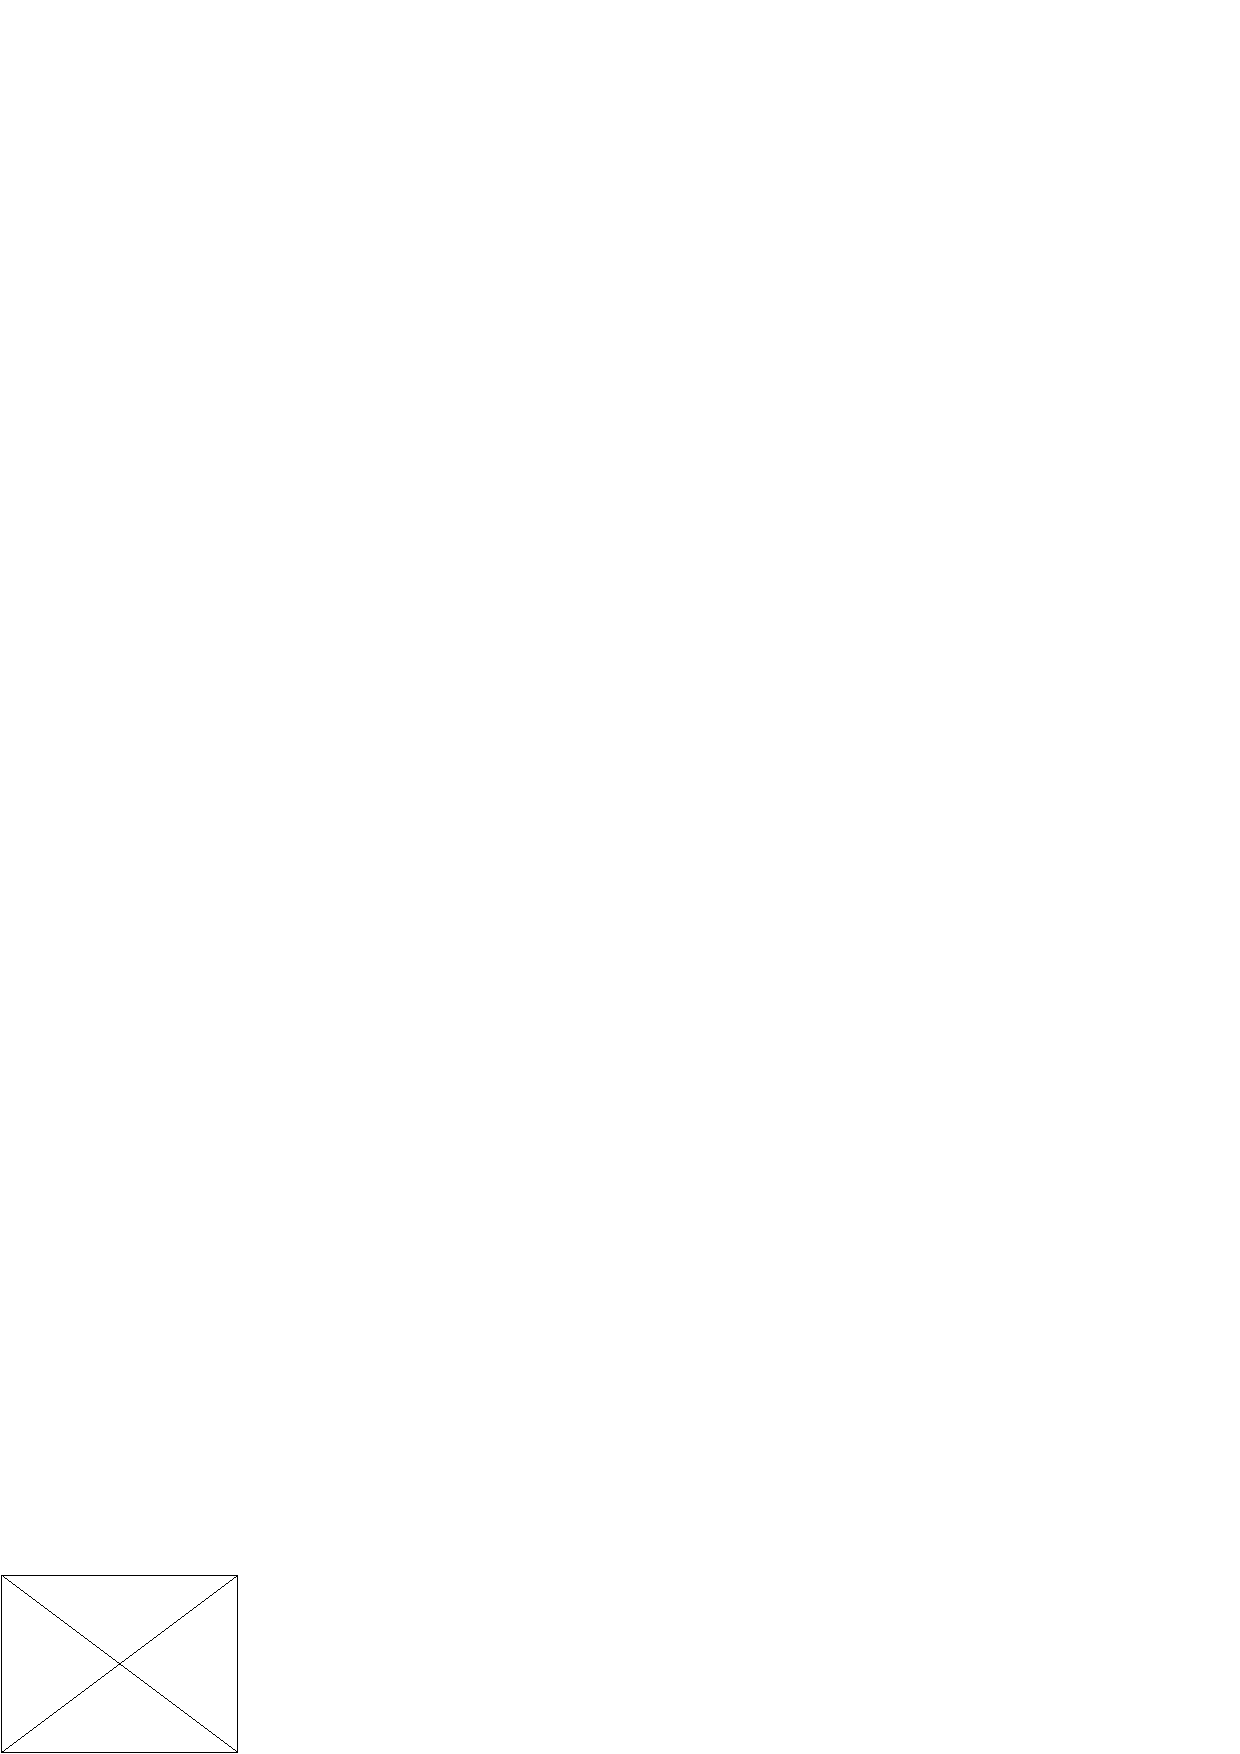
\includegraphics[width=66pt,height=86pt,draft]{empty}}{\textbf{Author Name.} This is sample author biography text this is sample author biography text this is sample author biography text this is sample author biography text this is sample author biography text this is sample author biography text this is sample author biography text this is sample author biography text this is sample author biography text this is sample author biography text this is sample author biography text this is sample author biography text this is sample author biography text this is sample author biography text this is sample author biography text this is sample author biography text this is sample author biography text this is sample author biography text this is sample author biography text this is sample author biography text this is sample author biography text.}
\end{biography}
\end{comment}
\end{document}
